\chapter{Обзор библиотеки DeepXDE}

DeepXDE (Deep Learning for Differential Equations)\cite{lu2021deepxde} –-- это открытая библиотека для Python,
предназначенная для решения различных типов дифференциальных уравнений с помощью методов
глубокого обучения. Она была разработана группой исследователей из Научно-технического
университета Китая и представлена в 2019 году. DeepXDE позволяет решать задачи, описываемые
обыкновенными и частными дифференциальными уравнениями, включая уравнения в частных производных и
уравнения с переменными коэффициентами.

Данная библиотека поддерживает следующие крупные библиотеки машинного обучения: tensorflow.compat.v1,
tensorflow, pytorch, jax, paddle.

\section{Возможности библиотеки}
Для постановки физической задачи необходимо четко определить, что рассматривается в качестве системы
(тело, частица, сплошная среда и т.д.), а также ее границы и взаимодействие с окружающей средой.
Следует задать начальное состояние системы, такое как начальное положение, скорость, температура,
давление и т.д. Необходимо определить, какие физические законы и принципы применимы к данной системе
(законы Ньютона, законы сохранения, принципы термодинамики и т.д.), и записать уравнения, описывающие
движение, взаимодействие или другие процессы в системе, на основе выбранных законов и принципов. При
необходимости нужно задать дополнительные условия, такие как связи, граничные условия, свойства
материалов и т.д. Также следует четко сформулировать, какие физические величины необходимо определить
в результате решения задачи. Этот минимум информации позволяет корректно сформулировать физическую
задачу и создать математическую модель для ее решения.

Суть метода заключается в использовании невязки всех уравнений, граничных и начальных условий в качестве
функции потерь. Это позволяет нейронной сети минимизировать данную ошибку и получить необходимый результат.

Невязка - это разница между левым и правым значениями уравнений. Она рассчитывается на основе начального решения,
которое задается случайным образом. Затем, с помощью методов минимизации функции потерь, решение уточняется.

Аналогичный метод решения мы можем видеть при численном решении системы линейных алгебраических уравнений (СЛАУ)
с помощью градиентного спуска. В этом случае, невязка также используется в качестве функции потерь, но минимизирует
ее градиентный спуск, чтобы получить решение СЛАУ.

Градиентный спуск - это один из наиболее распространенных методов минимизации функции потерь. Он заключается в том,
что на каждом шаге алгоритма мы изменяем решение в направлении, которое уменьшает значение функции потерь.

\subsection{Область}
Библиотека DeepXDE предоставляет ряд стандартных геометрических областей (geometry), которые можно применять к широкому
спектру задач. Некоторые из этих стандартных областей включают
\begin{minted}{python}
from deepxde.geometry.geometry_1d import Interval
from deepxde.geometry.geometry_2d import (
    Disk, Ellipse, Polygon, Rectangle, StarShaped, Triangle
)
from deepxde.geometry.geometry_3d import Cuboid, Sphere
from deepxde.geometry.geometry_nd import Hypercube, Hypersphere
from deepxde.geometry.timedomain  import GeometryXTime, TimeDomain
\end{minted}
Объекты данных, принадлежащие различным классам геометрических областей в библиотеке DeepXDE, наследуют функциональность
от базового интерфейсного класса deepxde.geometry.Geometry. Это позволяет им предоставлять следующие возможности:
\begin{enumerate}
    \item Проверка принадлежности точек: Определение, принадлежит ли заданная точка пространства данной геометрической
    области или ее границе.
    \item Вычисление нормали к границе: Вычисление направления нормального вектора к границе геометрической области в
    заданной точке.
    \item Операции над областями: Выполнение различных операций над геометрическими областями, таких как объединение,
    пересечение и определение их взаимного расположения.
    \item Генерация случайных точек: Получение набора случайных точек, равномерно распределенных внутри данной
    геометрической области или на ее границе.
\end{enumerate}
Эти универсальные методы, унаследованные от базового класса, позволяют использовать различные геометрические
области в широком спектре задач, решаемых с помощью библиотеки DeepXDE, обеспечивая согласованный и удобный
интерфейс для работы с пространственными данными и использованию области для решения дифференциальных уравнений.

К примеру, для моделирования задачи обтекания бесконечного цилиндра в DeepXDE, нам требуется определить следующую 
геометрическую область:
\begin{minted}{python}
base_domain = Rectangle(xmin=[0, 0], xmax=[3, 1])
barrier_domain = Ellipse(
    center=[0.5, 0.5], semimajor=0.1, semiminor=0.1
    )
space_domain = base_domain - barrier_domain

time_domain = dde.geometry.TimeDomain(0, 1)

domain = dde.geometry.GeometryXTime(space_domain, time_domain)
\end{minted}
Итак, мы определили геометрическую область, включающую базовый прямоугольник, эллиптический барьер, представляющий
собой поперечное сечение бесконечного цилиндра, и временную область. Эта геометрическая область будет использоваться
в дальнейшем примере для решения конкретной задачи.

\subsection{Уравнения}
Для задания дифференциальных уравнений или систем уравнений, которые описывают интересующую нас физическую,
мы можем использовать два специализированных оператора, предоставляемых библиотекой DeepXDE:
\begin{enumerate}
    \item deepxde.grad.jacobian: Этот оператор вычисляет якобиан заданной функции, что эквивалентно применению
    оператора набла.
    \item deepxde.grad.hessian: Этот оператор вычисляет гессиан заданной функции, что эквивалентно применению
    оператора Лапласа.
\end{enumerate}
Чтобы использовать эти уравнения или системы уравнений в дальнейшем процессе моделирования, нам необходимо создать
функцию, которая будет возвращать требуемые уравнения. Эта функция может быть затем применена к нашей ранее
определенной геометрической области для решения поставленной задачи.

Таким образом, мы можем гибко задавать необходимые дифференциальные уравнения, используя возможности библиотеки DeepXDE,
и интегрировать их в общий процесс моделирования и анализа.

Для моделирования двумерных гидродинамических процессов, мы можем воспользоваться уравнениями Навье-Стокса.
Эти фундаментальные дифференциальные уравнения в частных производных описывают движение вязких жидкостей и газов.

Пример реализации уравнений Навье-Стокса для двумерной задачи может выглядеть следующим образом:
\begin{minted}{python}
def navier_stocks(x, u):
    u_vel, v_vel, p = u[:, 0:1], u[:, 1:2], u[:, 2:3]

    u_vel_x = dde.grad.jacobian(u, x, i=0, j=0)
    u_vel_y = dde.grad.jacobian(u, x, i=0, j=1)
    u_vel_t = dde.grad.jacobian(u, x, i=0, j=2)
    u_vel_xx = dde.grad.hessian(u, x, component=0, i=0, j=0)
    u_vel_yy = dde.grad.hessian(u, x, component=0, i=1, j=1)

    v_vel_x = dde.grad.jacobian(u, x, i=1, j=0)
    v_vel_y = dde.grad.jacobian(u, x, i=1, j=1)
    v_vel_t = dde.grad.jacobian(u, x, i=1, j=2)
    v_vel_xx = dde.grad.hessian(u, x, component=1, i=0, j=0)
    v_vel_yy = dde.grad.hessian(u, x, component=1, i=1, j=1)

    p_x = dde.grad.jacobian(u, x, i=2, j=0)
    p_y = dde.grad.jacobian(u, x, i=2, j=1)

    momentum_x = (
        u_vel_t
        + (u_vel * u_vel_x + v_vel * u_vel_y)
        + p_x
        - 1 / Re * (u_vel_xx + u_vel_yy)
    )
    momentum_y = (
        v_vel_t
        + (u_vel * v_vel_x + v_vel * v_vel_y)
        + p_y
        - 1 / Re * (v_vel_xx + v_vel_yy)
    )
    continuity = u_vel_x + v_vel_y
    return [momentum_x, momentum_y, continuity]
\end{minted}

\subsection{Граничные и начальные условия}
В библиотеке DeepXDE (в подпространстве deepxde.icbc) имеется ряд классов, предназначенных для задания граничных условий задачи:
\begin{enumerate}
    \item DirichletBC: Задает граничные условия Дирихле, определяющие значение функции на границе.
    \item NeumannBC: Задает граничные условия Неймана, определяющие значение нормальной производной функции на границе.
    \item OperatorBC: Позволяет задавать граничные условия, определяемые произвольным дифференциальным оператором.
    \item RobinBC: Задает граничные условия Робина, комбинирующие условия Дирихле и Неймана.
    \item PeriodicBC: Используется для задания периодических граничных условий.
    \item PointSetBC: Позволяет задавать граничные условия, определенные на произвольном наборе точек.
    \item PointSetOperatorBC: Обобщение PointSetBC, где граничные условия определяются произвольным оператором.
\end{enumerate}
Каждый из этих классов позволяет не только задать соответствующее граничное условие, но и унаследовать или модифицировать
его с помощью дополнительных аргументов.

Аналогично, для задания начальных условий в DeepXDE используется класс IC, который позволяет определить начальное значение
решения в момент времени t=0.

Таким образом, библиотека DeepXDE предоставляет богатый набор инструментов для гибкого и точного задания граничных и начальных
условий при решении дифференциальных уравнений в частных производных.

При моделировании двумерной задачи гидродинамики на основе уравнений Навье-Стокса, мы можем задать следующие условия:

Граничные условия:
\begin{enumerate}
    \item На твердых стенках: Условие прилипания - скорость на границе равна нулю (условие Дирихле).
    \item На входной границе: Задаем профиль входной скорости (также условие Дирихле).
    \item На выходной границе: Используем условие Неймана, задавая нулевой градиент давления.
\end{enumerate}
Эти граничные условия можно реализовать в DeepXDE с помощью следующего кода:
\begin{minted}{python}
boundary_condition_inlet = dde.DirichletBC(
    domain, lambda x: 1,
    lambda x, on_boundary: 
    base_domain.on_boundary(x[0:2]) and np.isclose(x[0], 0.),
    component=0
)
boundary_condition_u = dde.DirichletBC(
    domain, lambda x: 0,
    lambda x, on_boundary: 
    base_domain.on_boundary(x[0:2]) 
    and (np.isclose(x[1], 0.) 
    and np.isclose(x[1], 1.)),
    component=0
)
boundary_condition_v = dde.DirichletBC(
    domain, lambda x: 0, 
    lambda x, on_boundary: base_domain.on_boundary(x[0:2]),
    component=1
)
barrier_condition_u = dde.DirichletBC(
    domain, lambda x: 0, 
    lambda x, on_boundary: barrier_domain.on_boundary(x[0:2]),
    component=0
)
barrier_condition_v = dde.DirichletBC(
    domain, lambda x: 0, 
    lambda x, on_boundary: barrier_domain.on_boundary(x[0:2]),
    component=1
)
barrier_condition_outlet = dde.NeumannBC(
    domain, lambda x: 0, 
    lambda x, on_boundary: 
    barrier_domain.on_boundary(x[0:2]) and np.isclose(x[0], 3.),
    component=2
)

initial_condition_u = dde.IC(
    domain, lambda x: 0,
    lambda x, on_initial: on_initial,
    component=0
)
initial_condition_v = dde.IC(
    domain, lambda x: 0,
    lambda x, on_initial: on_initial, 
    component=1
)
\end{minted}
    
\subsection{Создание модели}
Далее рассмотрим процесс создания модели с использованием библиотеки DeepXDE:
\begin{enumerate}
    \item Подготовка данных:
    Мы создаем объект dde.data.TimePDE(), который представляет собой временную задачу в частных производных.
    Этот объект принимает на вход определение области, дифференциальные уравнения,
    а также набор граничных и начальных условий.
    Мы также задаем количество точек данных для обучения и тестирования модели.
    \item Определение архитектуры сети:
    Для построения нейронной сети мы используем dde.nn.FNN(), создавая полносвязную сеть.
    Архитектура сети задается списком размеров слоев: [3] + 4 * [50] + [3], где 3 --- размер входного слоя, 4
    скрытых слоя по 50 нейронов, и 3 нейрона на выходе.
    Мы также указываем активационную функцию "tanh" и метод инициализации весов "Glorot normal".
    \item Создание модели:
    Объединяя подготовленные данные (data) и определенную архитектуру сети (net), мы создаем объект dde.Model(),
    представляющий собой полную модель.
\end{enumerate}
Такой процесс создания модели можно описать следующим образом в коде:
\begin{minted}{python}
data = dde.data.TimePDE(
    domain,
    navier_stocks,
    [
        boundary_condition_u,
        boundary_condition_v,
        initial_condition_u,
        initial_condition_v,
        barrier_condition_u,
        barrier_condition_v,
        barrier_condition_inlet,
        boundary_condition_outlet
    ],
    num_domain=50000,
    num_boundary=5000,
    num_initial=5000,
    num_test=10000,
)

net = dde.nn.FNN([3] + 4 * [50] + [3], "tanh", "Glorot normal")

model = dde.Model(data, net)    
\end{minted}
\subsection{Обучение модели}
Перед использованием этой модели необходимо выполнить следующие шаги:
\begin{enumerate}
    \item Выставить следующие параметры:
    \subitem Оптимизатор: "adam"
    \subitem Начальная скорость обучения: $10^{-3}$
    \subitem Веса потерь для различных компонентов целевой функции
    \item Начать обучение:
    \subitem Вызов метода model.train()
    \subitem Задание количества итераций обучения: $3000$
    \subitem Отображение информации о ходе обучения на каждой итерации
    \item После первого этапа обучения:
    \subitem Изменение оптимизатора на "L-BFGS"
    \subitem Повторный вызов model.train()
\end{enumerate}
Таким образом, код для обучения модели выглядит следующим образом:
\begin{minted}{python}
model.compile("adam", lr=1e-3, loss_weights=[...])
model.train(iterations=3000, display_every=1)
model.compile("L-BFGS", loss_weights=[...])
losshistory, train_state = model.train()
\end{minted}
Таким образом, модель проходит полный цикл предварительной настройки и обучения 
с использованием двух различных оптимизаторов.

Помимо обучения модели, предусмотрена возможность сохранения и загрузки существующей модели:
\begin{minted}{python}
model.train(model_save_path="model/")

model.restore("model/good_model.ckpt-43904.ckpt")    
\end{minted}
Таким образом, возможность сохранения и загрузки модели обеспечивает гибкость и эффективность в процессе работы с данной моделью.
\subsection{Применение модели}
Для создания эффективной модели необходимо тщательно подойти к выбору функции ошибки и оптимизатора, способного минимизировать 
эту функцию. Поскольку заранее нельзя гарантированно знать точную форму функции ошибки, приходится экспериментировать с различными
оптимизаторами.

В используемой библиотеке доступен широкий набор оптимизаторов из популярных API для нейронных сетей, таких как TensorFlow, PyTorch,
JAX и Paddle. Все они содержат как минимум оптимизаторы Adam и SGD.
Кроме того, библиотека DeepXDE предоставляет доступ к оптимизаторам L-BFGS и L-BFGS-B.

При обучении модели важно подобрать оптимальные весовые коэффициенты для различных компонентов целевой функции. Например, в представленных
примерах особый приоритет отдается выполнению граничных условий, поэтому им назначается высокий вес ($100$), а уравнению непрерывности - вес $10$.
Остальным компонентам можно присвоить вес $1$.

Такой подход к выбору оптимизатора и весовых коэффициентов позволяет достичь баланса между различными критериями качества модели и добиться
наилучших результатов.

Доступные оптимизаторы можно найти в документации к соответствующим API нейронных сетей: tensorflow.compat.v1 \cite{tfv1opt},
tensorflow \cite{tfopt}, pytorch \cite{pytorchopt}, jax \cite{jaxopt}, paddle \cite{paddleopt}.
\chapter{Результаты}
Все вычисления проводились на персональном компьютере и ноутбуке.
Системные характеристики персонального компьютера:
\begin{enumerate}
    \item Видеокарта: RTX 4080
    \item Процессор: Intel Core i9-14900KF
    \item Оперативная память: 64Gb DDR5 (2x32Gb)
\end{enumerate}
Системные характеристики ноутбука:
\begin{enumerate}
    \item Процессор: Ryzen 5 5500U
    \item Оперативная память: 16Gb DDR4 (2x8Gb)
\end{enumerate}
\begin{figure}
    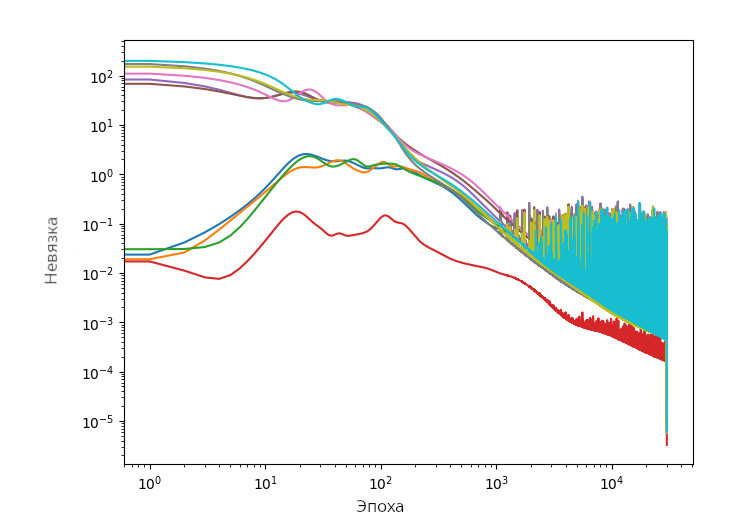
\includegraphics{course_work/error.png}
    \caption{Сходимость обучения модели для задачи трехмерного течения}
    \label{fig:error}
\end{figure}
% Рассмотрим подробнее подход к решению двух задач, где используются уравнения Навье-Стокса ---
% одна двумерная по обтеканию бесконечного цилиндра, другая трехмерная по потоку жидкости.

% \section{Первая задача}
% Дана квадратная замкнутая область со стороной 1. В центре этой области находится круговое препятствие в виде окружности радиусом 0.1.
% От левой стенки в данную область поступает жидкость со скоростью 1.
% Верхняя и нижняя стенки квадратной области являются твёрдыми непроницаемыми поверхностями.

% Для решения используем уравнение Навье-Стокса и поставим задачу следующим образом:
% \begin{equation}
%     \begin{cases}
%         u_t + (u\nabla)u = \frac{1}{Re} \Delta u \\
%         \nabla u = 0 \\
%         u(0, y) = 1 \\
%         u(1, y) = 1 \\
%         u(x, 0) = 0 \\
%         u(x, 1) = 0 \\
%         u_\Gamma = 0
%     \end{cases}
% \end{equation}
% В коде это будет выглядеть следующим образом (Приложение 1).
% Полученный результат представлен на (рис. \ref{fig:result}).
% \begin{figure}[ht]
%     \centering
%     \begin{minipage}{0.45\textwidth}
%         \centering
%         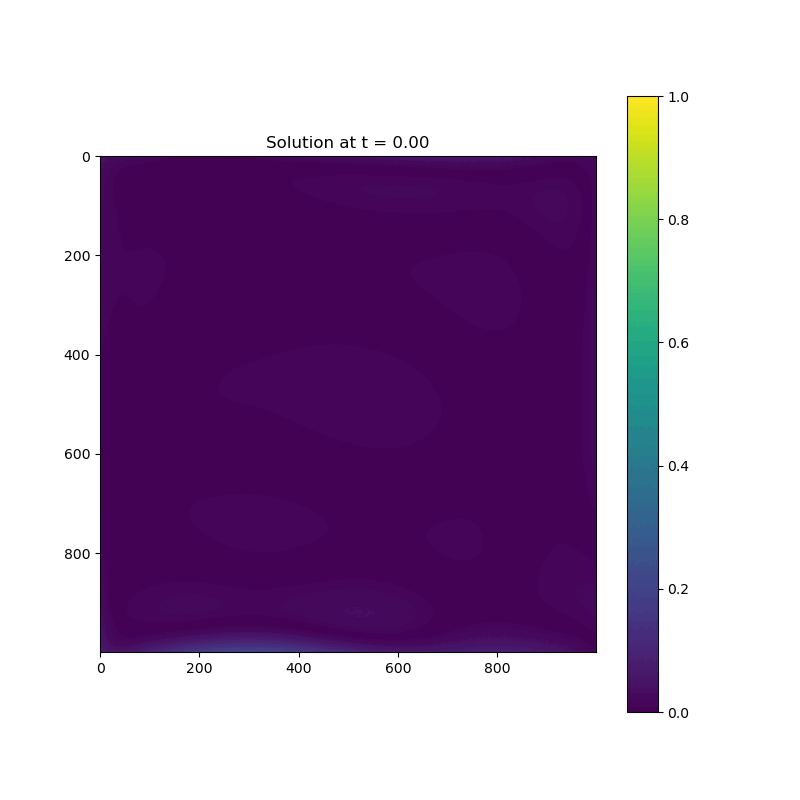
\includegraphics[width=\linewidth]{course_work/resalt_0.png}
%     \end{minipage}
%     \begin{minipage}{0.45\textwidth}
%         \centering
%         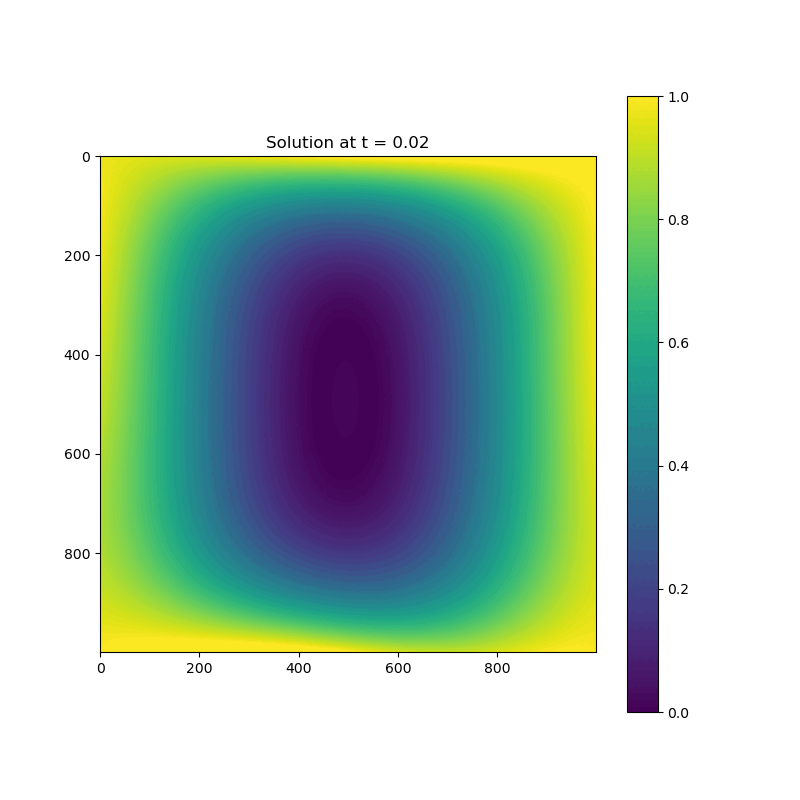
\includegraphics[width=\linewidth]{course_work/resalt_05.png}
%     \end{minipage}
%     \begin{minipage}{0.5\textwidth}
%         \centering
%         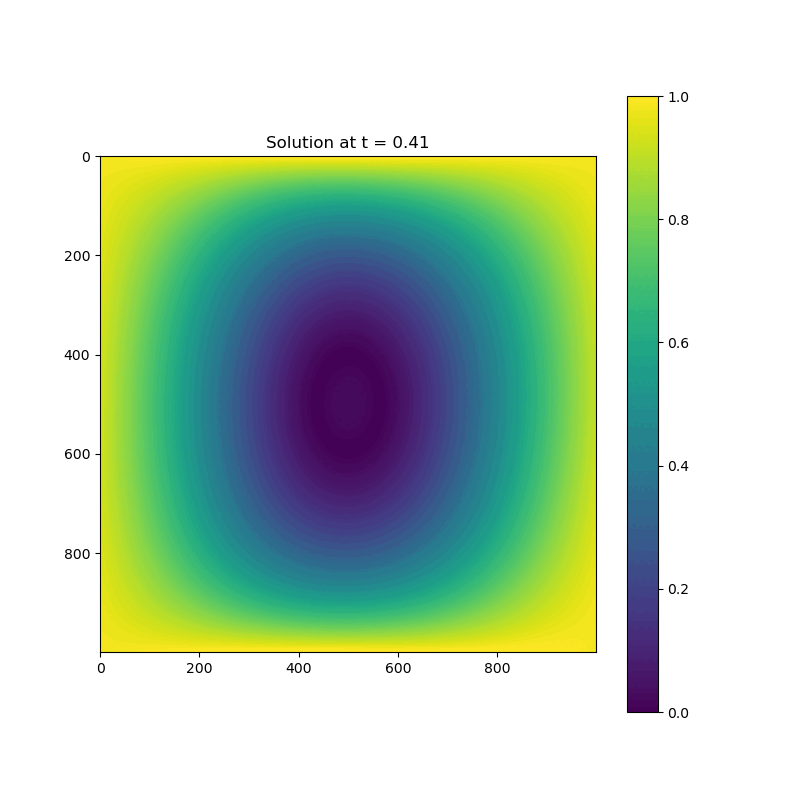
\includegraphics[width=\linewidth]{course_work/result_1.png}
%     \end{minipage}
%     \caption{Модуль скорости в разные моменты времени}
%     \label{fig:result}
% \end{figure}


% \section{Вторая задача}

% Для решения используем уравнение Навье-Стокса и поставим задачу следующим образом:
% \begin{equation}
%     \begin{cases}
%         u_t + (u\nabla)u = \frac{1}{Re} \Delta u \\
%         \nabla u = 0 \\
%         u(0, y) = 1 \\
%         u(1, y) = 1 \\
%         u(x, 0) = 0 \\
%         u(x, 1) = 0 \\
%         u_\Gamma = 0
%     \end{cases}
% \end{equation}
% В коде это будет выглядеть следующим образом (Приложение 1).
% Полученный результат представлен на (рис. \ref{fig:result}).
% \begin{figure}[ht]
%     \centering
%     \begin{minipage}{0.45\textwidth}
%         \centering
%         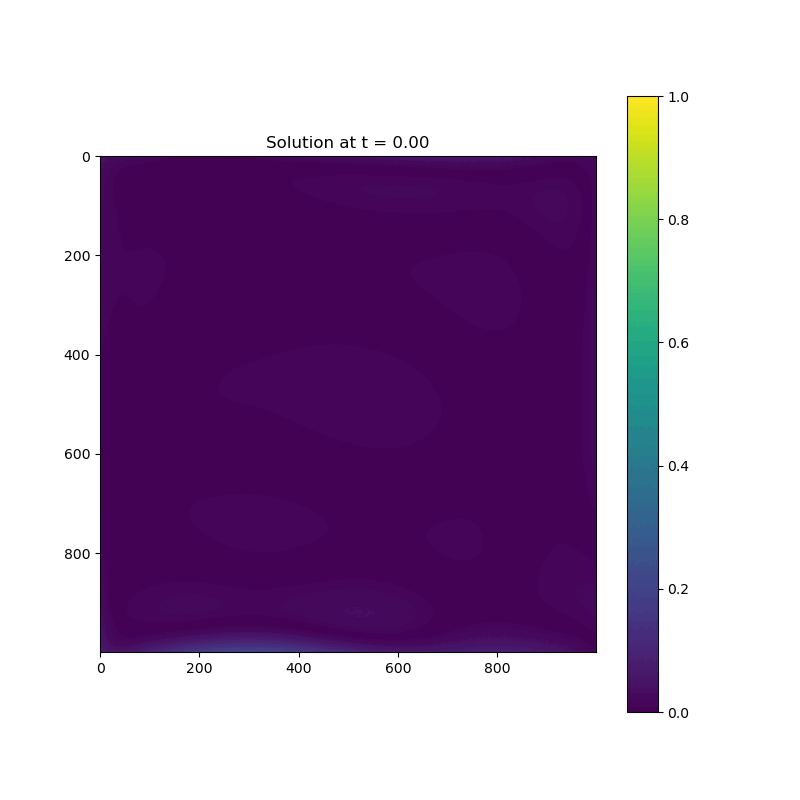
\includegraphics[width=\linewidth]{course_work/resalt_0.png}
%     \end{minipage}
%     \begin{minipage}{0.45\textwidth}
%         \centering
%         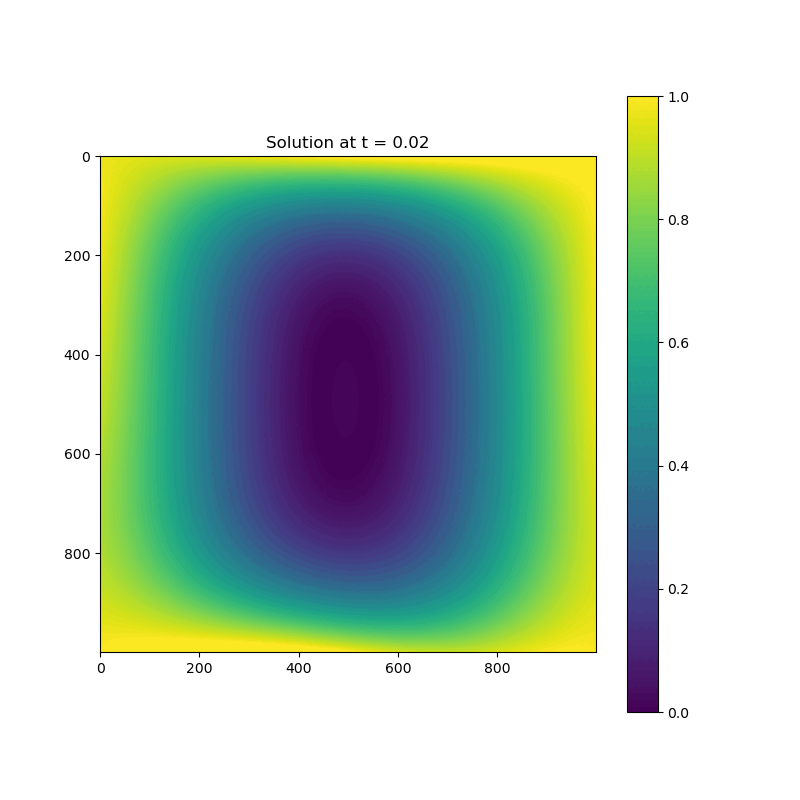
\includegraphics[width=\linewidth]{course_work/resalt_05.png}
%     \end{minipage}
%     \begin{minipage}{0.5\textwidth}
%         \centering
%         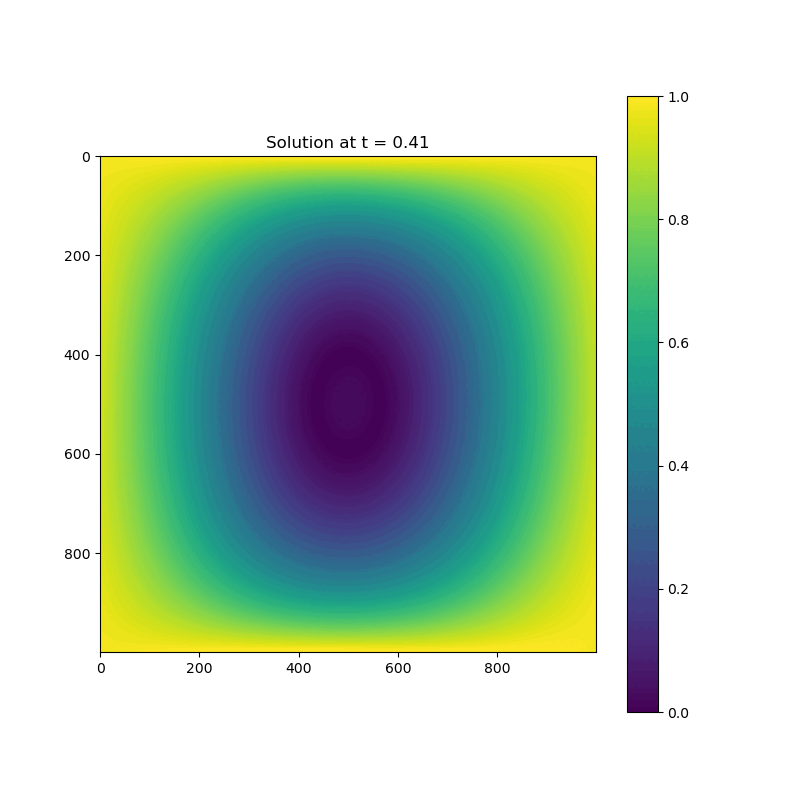
\includegraphics[width=\linewidth]{course_work/result_1.png}
%     \end{minipage}
%     \caption{Модуль скорости в разные моменты времени}
%     \label{fig:result}
% \end{figure}
Была решена следующая задача:
\begin{equation}
    \begin{cases}
        u_t + (u\nabla)u &= \nabla p-\frac{1}{Re} \Delta u \\
        \nabla u         &= 0 \\
        u(- 1, y, z, t)  &= -a \cdot (e^{-a} sin(a \cdot y + d \cdot z) + e^{a \cdot z}cos(-a + d \cdot y)) e^{-d^2t} \\
        u(1, y, z, t)    &= -a \cdot (e^{-a} sin(a \cdot y + d \cdot z) + e^{a \cdot z} cos(a + d \cdot y)) e^{-d^2t} \\
        v(x, - 1, z, t)  &= -a \cdot (e^{-a} sin(a \cdot z + d \cdot x) + e^{a \cdot x}cos(-a + d \cdot z)) e^{-d^2t} \\
        v(x, 1, z, t)    &= -a \cdot (e^{-a} sin(a \cdot z + d \cdot x) + e^{a \cdot x} cos(a + d \cdot z)) e^{-d^2t} \\
        w(x, y, - 1, t)  &= -a \cdot (e^{-a} sin(a \cdot x + d \cdot y) + e^{a \cdot y}cos(-a + d \cdot x)) e^{-d^2t} \\
        w(x, y, 1, t)    &= -a \cdot (e^{-a} sin(a \cdot x + d \cdot y) + e^{a \cdot y} cos(a + d \cdot x)) e^{-d^2t} \\

        u(x, y, z, 0)    &= -a \cdot (e^{a \cdot x} \cdot sin(a \cdot y + d \cdot z) + e^{a \cdot z} cos(a \cdot x + d \cdot y)) \\
        v(x, y, z, 0)    &= -a \cdot (e^{a \cdot y} \cdot sin(a \cdot z + d \cdot x) + e^{a \cdot z} cos(a \cdot y + d \cdot z)) \\
        w(x, y, z, 0)    &= -a \cdot (e^{a \cdot z} \cdot sin(a \cdot x + d \cdot y) + e^{a \cdot z} cos(a \cdot z + d \cdot x)) \\
    \end{cases}
\end{equation}

Обучение трехмерной модели на персональном компьютере потребовало значительных ресурсов - $4$ часа $51$ минут и $30000$
итераций. Однако, использование GPU позволило существенно ускорить процесс, сократив время обучения до $55$ минут $41$
секунды, что почти в $5$ раз эффективнее. Эти результаты демонстрируют важность оптимизации вычислительных ресурсов
для повышения производительности обучения нейронной сети.

Кроме того, был проведен анализ точности обученной модели. Как видно из рисунка \ref{fig:error}, ошибки
аппроксимации по каждому из уравнений находятся на приемлемом уровне. Более того, вычисленные относительные погрешности
по сравнению с аналитическим решением также подтверждают высокую точность модели - на момент времени $t=0$ максимальная
погрешность составляет около $0.04\%$, а на момент $t=1$ - не более $0.18\%$.

Таким образом, полученные результаты свидетельствуют о том, что данная нейронная сеть способна
эффективно и точно решать трехмерные задачи гидродинамики, что делает ее перспективным инструментом для широкого круга
практических применений. Дальнейшие эксперименты на ноутбуке позволят детально исследовать производительность и масштабируемость данного подхода.

\begin{figure}[h]
    \center
    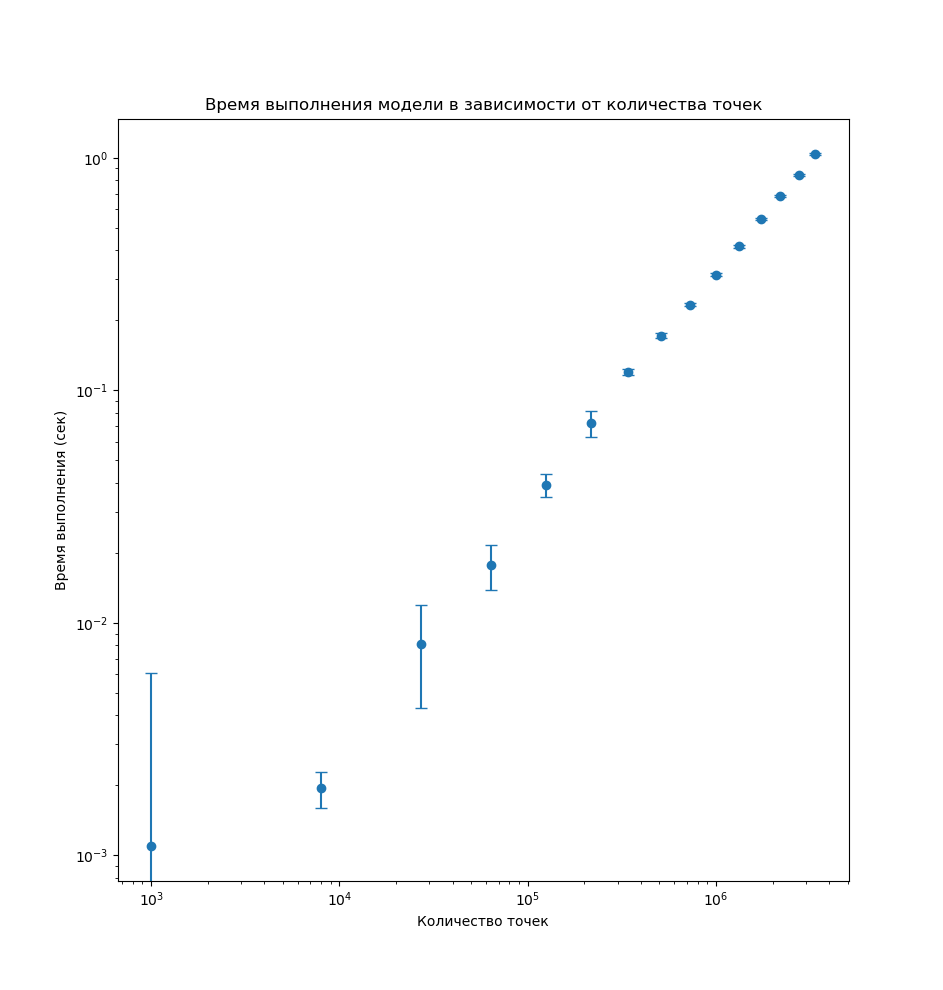
\includegraphics[width=0.8\textwidth]{course_work/speed_calculation.png}
    \caption{Скорость предсказания решения}
    \label{fig:speed}
\end{figure}
Представленное исследование демонстрирует значительные преимущества использования физически информированных нейронных сетей 
в сочетании с библиотекой DeepXDE для решения задач гидродинамики. Одним из ключевых показателей эффективности данного 
подхода является время вычисления решения.

Из рисунка \ref{fig:speed} видно, что для сетки размерности 10x10x10 (1000 точек) и 60 временных шагов, решение PINN может быть
получено всего за 0.0943 секунды. Этот результат особенно впечатляет, учитывая, что такое быстрое вычисление решения делает метод
идеально подходящими для использования на слабых вычислительных устройствах.

Таким образом, данная работа не только подтверждает эффективность метода в моделировании гидродинамических процессов,
но и демонстрирует, насколько сильно данный подход может упростить и ускорить получение решений. Это открывает новые возможности
для применения данного метода в различных областях, где требуется быстрая симуляция.

Дальнейшие исследования в этом направлении могут быть сосредоточены на расширении применимости PINN к более сложным трехмерным задачам,
а также на разработке новых методик обучения для улучшения масштабируемости и скорости сходимости. Общий вклад данной работы
заключается в продвижении методов численного моделирования с использованием передовых инструментов машинного обучения.
\chapter{Использование NPU для ускорения работы модели}
NPU (Neural Process Unit) является вспомогательным процессором, предназначенным для ускорения тензорных операций, 
необходимых для работы нейронных сетей. Такой специализированный процессор очень удобно применять для получения результатов 
нейронных сетей в режиме реального времени.

В настоящее время NPU есть практически в каждом современном мобильном устройстве, поскольку он необходим для решения таких 
задач, как распознавание лиц, обнаружение людей на камере, обработка фото и видео. Операционные системы предоставляют API, 
позволяющий напрямую взаимодействовать с NPU для использования моделей TensorFlow Lite, которые можно экспортировать из TensorFlow\cite{nnapi}.

Такой подход открывает широкие возможности для реалистичного моделирования физических процессов в режиме реального времени,
как в научных целях, так и для мобильных игр. Это позволяет разгрузить центральный процессор (CPU) и использовать его
вычислительные мощности для других задач.

Для реализации мобильных приложений с использованием NPU существует три основных подхода:
\begin{enumerate}
    \item Используя Java или Kotlin (только для Android)
    \item Используя Objective-C++ или Swift (только для iOS)
    \item Используя C++ NDK (любое устройство с возможностью использовать NPU)
\end{enumerate} 

Из этих вариантов наиболее предпочтительным является использование C++, так как это кроссплатформенный подход,
который особенно хорошо подходит для игр и симуляций на мобильных устройствах.

Использование C++ NDK (Native Development Kit) позволяет разработчикам взаимодействовать напрямую с NPU (Neural Process Unit) на мобильных устройствах, как на Android, так и на iOS.
\begin{enumerate}
    \item 
    Android:
    \subitem
    В Android, начиная с версии 9.0 (Pie), доступен API Android Neural Networks (NNAPI), который позволяет использовать NPU
    для ускорения вычислений нейронных сетей.
    Для использования NNAPI в C++ приложениях на Android, разработчики могут воспользоваться библиотекой TensorFlow Lite C++ API.
    Это позволяет эффективно интегрировать модели TensorFlow Lite в C++ код и задействовать аппаратное ускорение NPU.
    Дополнительно, Android предоставляет API Android Runtime (ART), который также можно использовать для взаимодействия с NPU через C++ NDK.
    \item
    iOS:
    \subitem
    На iOS, начиная с версии 12, доступен фреймворк Core ML, который позволяет использовать NPU (известный как "Neural Engine" на iOS) 
    для ускорения вычислений с нейронными сетями.
    Для интеграции Core ML в C++ приложения на iOS, разработчики могут воспользоваться библиотекой TensorFlow Lite C++ API. Это дает 
    возможность эффективно использовать модели TensorFlow Lite и задействовать возможности iOS Neural Engine.
    Кроме того, iOS предоставляет низкоуровневый API Metal Performance Shaders (MPS), который также может быть использован для прямого взаимодействия
    с NPU через C++ код.
    Использование C++ NDK вместе с TensorFlow Lite C++ API или другими низкоуровневыми API позволяет разработчикам максимально
    эффективно использовать возможности NPU на мобильных устройствах Android и iOS. Это особенно важно для приложений, требующих
    высокой производительности в режиме реального времени, таких как мобильные игры, симуляции физических процессов, компьютерное зрение и т.д.
\end{enumerate}

\chapter{Заключение}
В данной работе была продемонстрирована эффективность использования физически информированных нейронных сетей для решения задач гидродинамики с помощью библиотеки DeepXDE.
Несмотря на то, что библиотека DeepXDE продолжает развиваться, на данный момент она гарантирует качество результатов только при использовании API Paddle.
Это ограничивает возможности применения более популярного API TensorFlow, что не позволяет в полной мере раскрыть потенциал нейронной сети и добиться наилучших
результатов при обучении. Вместе с тем, физически-информированные нейронные сети являются относительно простыми в реализации, и их можно построить вручную,
используя любой API для обучения нейронных сетей. 
Физически-информированные нейронные сети представляют собой гибкий и мощный подход, который позволяет включать физические законы и условия в процесс обучения нейронных сетей.

Ключевыми преимуществами использования PINN для гидродинамических задач являются:
\begin{enumerate}
    \item Учитывание физических законов.
    Физически-информированные нейронные сети позволяют напрямую включать уравнения Навье-Стокса и граничные условия в архитектуру нейронной сети, что обеспечивает физическую достоверность решений.
    \item Эффективное использование данных: 
    Физически-информированные нейронные сети могут обучаться на относительно небольших наборах данных, поскольку физические законы используются для ограничения пространства решений.
    \item Средняя точность и гладкость решений: 
    Благодаря использованию автоматического дифференцирования, физически-информированные нейронные сети способны давать точные и гладкие решения, что важно для многих гидродинамических приложений.
    \item Универсальность: 
    Подход PINN может быть применен к широкому спектру гидродинамических задач, включая течения в каналах, обтекание тел, вихревые течения и многое другое.
    \item Простота реализации:
    Для реализации физически-информированных нейронных сетей с помощью библиотеки DeepXDE не нужно особых знаний в области численных методов, достаточно понимать структуру нейронных сетей.
    \item Легкий перенос решения:
    Для переноса решения достаточно сохранить модель и ее дальше можно дообучать и использовать, не тратя время на повторное обучение. Также такое решение весьма легковесно для использования
    в играх или микроконтроллерах
\end{enumerate}
Результаты, представленные в этом исследовании, демонстрируют, что физически-информированные нейронные сети в сочетании с DeepXDE являются многообещающим подходом для эффективного
моделирования гидродинамических процессов. Дальнейшие исследования в этом направлении могут включать применение физически-информированных нейронных сетей к более сложным трехмерным задачам,
а также разработку новых архитектур и методик обучения для улучшения масштабируемости и скорости сходимости.

К такому подходу идеально применяется многопроцессорность, что позволяет считать такие модели, как на одном процессоре, так и на кластере из процессоров и видеокарт, что может ускорить 
процесс обучения.

В ряде случаев, например в мобильных играх, можно применять NPU для ускорения получения результатов, что актуально для всех современных телефонов. Такой подход полностью убирает
необходимость использовать CPU для расчетов физики в играх, что является хорошей оптимизацией. 